\documentclass[a4paper, 12pt]{article}

\usepackage{amsmath, amsthm}

\usepackage{unicode-math}
\usepackage{xltxtra}
\usepackage{xgreek}
\setmainfont{Calibri}

\usepackage[margin=1.2cm]{geometry}

\usepackage[most]{tcolorbox}

\tcbuselibrary{listingsutf8}
\tcbset{
  theoremstyle/.style={
    colback=blue!5!white,
    colframe=blue!75!black,
    fonttitle=\bfseries,
    coltitle=black,
    colbacktitle=blue!10!white,
    enhanced,
    attach boxed title to top left={xshift=2mm,yshift=-2mm}
  },
}

\newtcolorbox[auto counter]{theorem}[2][]{%
  theoremstyle,
  title={Ορισμός~\thetcbcounter: #2}, #1
}

\title{Ορισμοί Γ' Λυκείου}
\author{Κωνσταντίνος Λόλας}
\date{2025}

\usepackage{imakeidx}
\usepackage{hyperref}
\makeindex

\begin{document}

\maketitle

\begin{theorem}{Συνάρτηση}
  Έστω $Α$ ένα υποσύνολο του $\mathbb{R}$. Τι ονομάζουμε πραγματική συνάρτηση με πεδίο ορισμού το $Α$;
\end{theorem}
\begin{proof}
  Ονομάζουμε πραγματική συνάρτηση\index{Συνάρτηση} με πεδίο ορισμού το $Α$ μια διαδικασία (κανόνα) $f$, με την οποία κάθε στοιχείο $\in Α$ αντιστοιχίζεται σε ένα μόνο πραγματικό αριθμό $y$. Το $y$ ονομάζεται τιμή της $f$ στο $x$ και συμβολίζεται με $f(x)$.
\end{proof}

\begin{theorem}{Γραφική Παράσταση}
  Τι ονομάζουμε γραφική παράσταση μιας συνάρτησης $f$;
\end{theorem}
\begin{proof}
  Έστω $f$ μια συνάρτηση με πεδίο ορισμού $Α$ και $Oxy$ ένα σύστημα συντεταγμένων στο επίπεδο. Το σύνολο των σημείων $M(x, y)$ για τα οποία ισχύει $y = f(x)$, δηλαδή το σύνολο των σημείων $M(x, f(x))$, $x \in A$, λέγεται γραφική παράσταση\index{Γραφική Παράσταση} της $f$ και συμβολίζεται συνήθως με $C_f$.
\end{proof}

\begin{theorem}{Ισότητα Συναρτήσεων}
  Πότε λέμε ότι δύο συναρτήσεις $f$ και $g$ είναι ίσες;
\end{theorem}
\begin{proof}
  Δύο συναρτήσεις $f$ και $g$ λέγονται ίσες\index{Ισότητα Συναρτήσεων} όταν:
  \begin{itemize}
    \item έχουν το ίδιο πεδίο ορισμού $Α$ και
    \item για κάθε $x \in A$ ισχύει $f(x) = g(x)$.
  \end{itemize}
\end{proof}

\begin{theorem}{Πράξεις Συναρτήσεων}
  Έστω $f$ και $g$ δύο συναρτήσεις ορισμένες στα $Α$ και $Β$ αντίστοιχα. Πώς ορίζονται οι πράξεις άθροισμα, διαφορά, γινόμενο και πηλίκο των συναρτήσεων $f$ και $g$;
\end{theorem}
\begin{proof}
  Ορίζουμε\index{Πράξεις Συναρτήσεων} ως άθροισμα $f + g$,  διαφορά $f - g$,  γινόμενο $fg$  και  πηλίκο $\dfrac{f}{g}$ δύο συναρτήσεων $f$, $g$ τις συναρτήσεις με τύπους:
  \begin{itemize}
    \item $(f + g)(x) = f(x) + g(x)$
    \item $(f - g)(x) = f(x) - g(x)$
    \item $(fg)(x) = f(x)g(x)$
    \item $\left(\dfrac{f}{g}\right)(x) = \dfrac{f(x)}{g(x)}$.
  \end{itemize}
  Το πεδίο ορισμού των $f+g$, $f-g$, $fg$ είναι η τομή $A \cap B$ των πεδίων ορισμού των συναρτήσεων $f$ και $g$, ενώ το πεδίο ορισμού της $\frac{f}{g}$ είναι το $A \cap B$ εξαιρουμένων των τιμών του $x$ που μηδενίζουν τον παρανομαστή $g$. δηλαδή
  $$ \{ x|x\in A \cap B, g(x) \neq 0 \}$$
\end{proof}

\begin{theorem}{Σύνθεση Συναρτήσεων}
  Έστω $f$ και $g$ δύο συναρτήσεις ορισμένες στα $A$ και $B$ αντίστοιχα. Πώς ορίζεται η σύνθεση των συναρτήσεων $f$ και $g$;
\end{theorem}
\begin{proof}
  Αν $f$, $g$ είναι δύο συναρτήσεις με πεδίο ορισμού $Α$, $Β$ αντιστοίχως, τότε ονομάζουμε σύνθεση\index{Σύνθεση Συναρτήσεων} της $f$ με την $g$, και τη συμβολίζουμε με $g\circ f$, τη συνάρτηση με τύπο

  $$(g\circ f)(x) = g(f(x))$$


  \begin{center}
    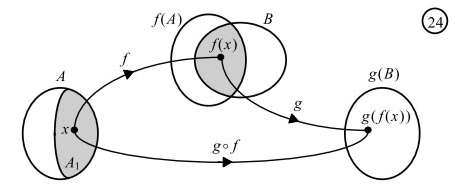
\includegraphics[width=0.5\textwidth]{images/1.2 Σύνθεση}
  \end{center}

  Το πεδίο ορισμού της $g\circ f$ αποτελείται από όλα τα στοιχεία $x$ του πεδίου ορισμού της $f$ για τα οποία το $f(x)$ ανήκει στο πεδίο ορισμού της $g$. Δηλαδή είναι το σύνολο
  $A_1 = \{ x \in A   |   f(x) \in Β\}$
\end{proof}

\begin{theorem}{Γνησίως Αύξουσα Συνάρτηση}
  Πότε μια συνάρτηση $f$ λέγεται γνησίως αύξουσα σε ένα διάστημα $Δ$;
\end{theorem}
\begin{proof}
  Μια συνάρτηση $f$ λέγεται γνησίως αύξουσα\index{Γνησίως Αύξουσα Συνάρτηση} σε ένα διάστημα $Δ$ αν για κάθε $x_1, x_2 \in Δ$ με $x_1 < x_2$ ισχύει $f(x_1) < f(x_2)$.
\end{proof}

\begin{theorem}{Γνησίως Φθίνουσα Συνάρτηση}
  Πότε μια συνάρτηση $f$ λέγεται γνησίως φθίνουσα σε ένα διάστημα $Δ$;
\end{theorem}
\begin{proof}
  Μια συνάρτηση $f$ λέγεται γνησίως φθίνουσα\index{Γνησίως Φθίνουσα Συνάρτηση} σε ένα διάστημα $Δ$ αν για κάθε $x_1, x_2 \in Δ$ με $x_1 < x_2$ ισχύει $f(x_1) > f(x_2)$.
\end{proof}

\begin{theorem}{Αύξουσα Συνάρτηση}
  Πότε μια συνάρτηση $f$ λέγεται αύξουσα σε ένα διάστημα $Δ$;
\end{theorem}
\begin{proof}
  Μια συνάρτηση $f$ λέγεται αύξουσα\index{Αύξουσα Συνάρτηση} σε ένα διάστημα $Δ$ αν για κάθε $x_1, x_2 \in Δ$ με $x_1 < x_2$ ισχύει $f(x_1) \leq f(x_2)$.
\end{proof}

\begin{theorem}{Φθίνουσα Συνάρτηση}
  Πότε μια συνάρτηση $f$ λέγεται φθίνουσα σε ένα διάστημα $Δ$;
\end{theorem}
\begin{proof}
  Μια συνάρτηση $f$ λέγεται φθίνουσα\index{Φθίνουσα Συνάρτηση} σε ένα διάστημα $Δ$ αν για κάθε $x_1, x_2 \in Δ$ με $x_1 < x_2$ ισχύει $f(x_1) \geq f(x_2)$.
\end{proof}

\begin{theorem}{Γνησίως Μονότονη Συνάρτηση}
  Πότε μια συνάρτηση $f$ λέγεται γνησίως μονότονη σε ένα διάστημα $Δ$;
\end{theorem}
\begin{proof}
  Μια συνάρτηση $f$ λέγεται γνησίως μονότονη\index{Γνησίως Μονότονη Συνάρτηση} σε ένα διάστημα $Δ$ αν είναι γνησίως αύξουσα ή γνησίως φθίνουσα σε αυτό.
\end{proof}

\begin{theorem}{Μέγιστο}
  Πότε μια συνάρτηση $f$ με πεδίο ορισμού το $A$ θα λέμε ότι έχει μέγιστο στο $x_0$;
\end{theorem}
\begin{proof}
  Έστω $f$ μια συνάρτηση με πεδίο ορισμού το $A$. Θα λέμε ότι η $f$ παρουσιάζει στο $x_0\in Α$ μέγιστο\index{Μέγιστο} το $f(x_0)$ αν ισχύει:
  $$f(x_0) \geq f(x) \quad \forall x \in A$$
\end{proof}

\begin{theorem}{Ελάχιστο}
  Πότε μια συνάρτηση $f$ με πεδίο ορισμού το $A$ θα λέμε ότι έχει ελάχιστο στο $x_0$;
\end{theorem}
\begin{proof}
  Έστω $f$ μια συνάρτηση με πεδίο ορισμού το $A$. Θα λέμε ότι η $f$ παρουσιάζει στο $x_0\in Α$ ελάχιστο\index{Ελάχιστο} το $f(x_0)$ αν ισχύει:
  $$f(x_0) \leq f(x) \quad \forall x \in A$$
\end{proof}

\begin{theorem}{Ακρότατο}
  Τι ονομάζουμε ακρότατα μιας συνάρτησης $f$;
\end{theorem}
\begin{proof}
  Το μέγιστο και το ελάχιστο μιας συνάρτησης $f$ λέγονται ακρότατα\index{Ακρότατα} της $f$.
\end{proof}

\begin{theorem}{1-1}
  Πότε μια συνάρτηση $f$ λέγεται 1-1;
\end{theorem}
\begin{proof}
  Μια συνάρτηση $f$ λέγεται 1-1\index{1-1} αν για κάθε $x_1, x_2 \in A$ με $x_1 \neq x_2$ ισχύει $f(x_1) \neq f(x_2)$.
\end{proof}

\begin{theorem}{Αντίστροφη Συνάρτηση\index{Αντίστροφη}}
  Πώς ορίζεται η αντίστροφη συνάρτηση μιας $f$;
\end{theorem}
\begin{proof}
  Έστω μια συνάρτηση $f : A \to \mathbb{R}$. Αν υποθέσουμε ότι αυτή είναι 1–1, τότε για κάθε στοιχείο $y$ του συνόλου τιμών, $f(A)$, της $f$ υπάρχει μοναδικό στοιχείο $x$ του πεδίου ορισμού της $Α$ για το οποίο ισχύει $f(x) = y$. Επομένως ορίζεται μια συνάρτηση
  $g : f ( A) \to \mathbb{R}$ με την οποία κάθε $y \in f ( A)$ αντιστοιχίζεται στο μοναδικό $x \in A$ για το οποίο ισχύει $f(x) = y$.
\end{proof}

\begin{theorem}{Κριτήριο Παρεμβολής\index{Κριτήριο Παρεμβολής}}
  Να διατυπώσετε το κριτήριο παρεμβολής
\end{theorem}
\begin{proof}
  Έστω οι συναρτήσεις $f$, $g$, $h$. Αν
  \begin{itemize}
    \item $h(x) \leq f(x) \leq g(x)$ για κάθε $x$ κοντά στο $x_0$ και
    \item $\lim_{x \to x_0} h(x) = \lim_{x \to x_0} g(x) = λ$,
  \end{itemize}
  τότε
  $$\lim_{x \to x_0} f(x) = λ$$
\end{proof}

\begin{theorem}{Ακολουθία\index{Ακολουθία}}
  Να δώσετε τον ορισμό της ακολουθίας.
\end{theorem}
\begin{proof}
  Ακολουθία ονομάζεται κάθε πραγματική συνάρτηση $α : \mathbb{N} \to \mathbb{R}$.
\end{proof}

\begin{theorem}{Συνέχεια σε σημείο\index{Συνέχεια σε σημείο}}
  Να δώσετε τον ορισμό της συνέχειας σε σημείο $x_0$.
\end{theorem}
\begin{proof}
  Έστω μια συνάρτηση $f$ και $x_0$ ένα σημείο του πεδίου ορισμού της. Θα λέμε ότι η $f$ είναι συνεχής στο $x_0$, όταν
  $$\lim_{x \to x_0} f(x) = f(x_0)$$
\end{proof}

\begin{theorem}{Συνέχεια σε ανοιχτό διάστημα\index{Συνέχεια σε ανοιχτό διάστημα}}
  Πότε λέμε ότι μια συνάρτηση 𝑓 είναι συνεχής σε ένα ανοικτό διάστημα  $(α, β)$;
\end{theorem}
\begin{proof}
  Μια συνάρτηση $f$ θα λέμε ότι είναι συνεχής σε ένα ανοικτό διάστημα $(α, β)$, όταν είναι συνεχής σε κάθε σημείο του $(α, β)$
\end{proof}

\begin{theorem}{Συνέχεια σε κλειστό διάστημα\index{Συνέχεια σε κλειστό διάστημα}}
  Πότε λέμε ότι μια συνάρτηση 𝑓 είναι συνεχής σε ένα κλειστό διάστημα  $[α, β]$;
\end{theorem}
\begin{proof}
  Μια συνάρτηση $f$ θα λέμε ότι είναι συνεχής σε ένα κλειστό διάστημα $[α, β]$, όταν είναι συνεχής στο ανοιχτό $(α, β)$ και επιπλέον
  \begin{itemize}
    \item $\lim_{x \to α^+} f(x) = f(α)$
    \item $\lim_{x \to β^-} f(x) = f(β)$
  \end{itemize}
\end{proof}


\printindex

\end{document}